\chapter{Metodi Harvesting Energetico}

\begin{section}{Sorgenti Corporee}
   Movimento, vibrazioni, gradienti di temperatura e reazioni enzimatiche possono essere convertiti in energia elettrica da harvester. L'attivita' fisica e i processi fisiologici offrono fonti energetiche con intensita' irregolare ma sempre accessibile. Per alcuni movimenti e' anche possibile raccogliere il lavoro necessario alla frenata, riducendo addirittura il costo metabolico dell'azione \cite{liuBiomechanicalEnergyHarvesting2022}. In particolare un livello basale di energia meccanica dovuto al movimento e' sempre disponibile, cosi' come l'energia chimica immagazzinata nei liquidi corporei.
   
   \begin{subsection}{Generatori Triboelettrici}
    Un generatore triboelettrico sfrutta materiali che si caricano elettricamente strisciando l'uno sull'altro. In base alla capacita' di generare una densita' di carica al contatto o sfregamento, sono organizzati nella serie triboelettrica \cite{zouQuantifyingTriboelectricSeries2019}. E' una proprieta' presente anche in molti materiali organici e leggeri. Quando stimolati producono alte tensioni e basse correnti per piccoli istanti di tempo. Usare piu' strati di materiali aumenta la potenza prodotta. Le migliori zone di applicazione sono negli arti inferiori, dove si sviluppano le forze maggiori, come nella pianta del piede.
    \begin{figure}[H]
        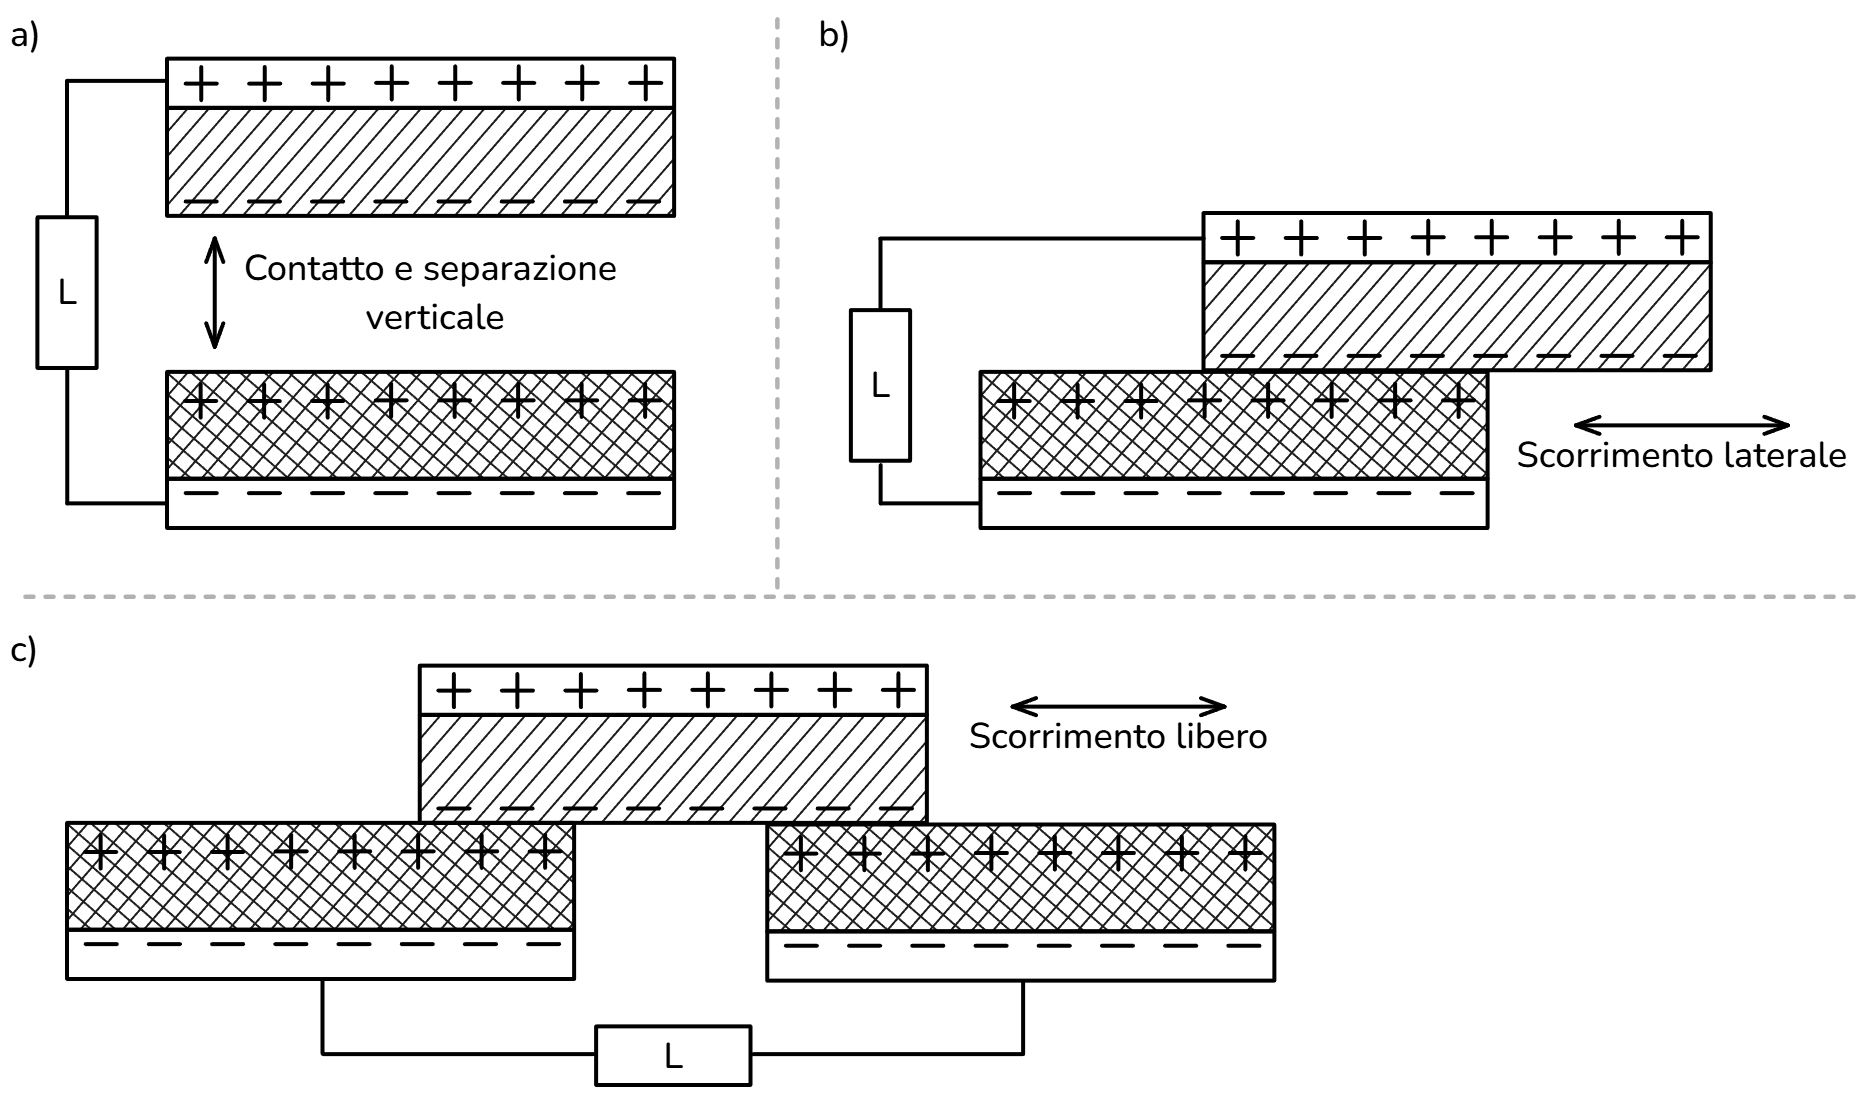
\includegraphics[width=1\textwidth]{triboelettrici.png}
        \centering
        \caption{a) Generatore triboelettrico a contatto verticale. b) Generatore triboelettrico a scorrimento laterale. c)Generatore triboelettrico a scorrimento libero.}
        \label{fig:triboelettrici}
    \end{figure}
   \end{subsection}

   \begin{subsection}{Generatori Piezoelettrici}
    I sistemi di harvesting piezoelettrici producono energia elettrica attraverso la deformazione elastica di materiali piezoelettrici. Quando l'elasticita' del materiale stesso e' insufficiente, lo si puo' integrare ad altri materiali con migliori proprieta' meccaniche. Possono essere di forma e dimensione arbitraria, inoltre usano materiali leggeri, poco costosi, non tossici e anche facili da assemblare. Producono corrente anche per stimoli molto piccoli, ma la potenza e' bassa cosi' come l'efficienza. Lo studio di materiali flessibili e' una possibile soluzione dato che permetterebbero l'installazzione in zone del corpo che subiscono forze maggiori. In mancanza di stimoli prevalenti si ha una conversione dell'energia meccanica data dalle vibrazioni. Le performance di elementi ottenuti da pellicole di materiale sono inferiori ai tessuti di fibre. Il polivinildenfluoro PVDF abbinato a vari additivi e' il polimero piu' usato negli studi. La quantita' di energia generata dipende dal posizionamento dell'harvester e dallo stato di attivita' fisica. Gli arti inferiori sono sottoposti a forze maggiori, specilamente durante il cammino. Posizionare il generatore in una suola o accoppiarlo alla flessione del ginocchio offre i risultati migliori in termini di potenza. La tecnologia piezoelettrica e' pero' anche valida come sensoristica attiva di pressione. Sensori di questo tipo possono essere usati per monitorare la respirazione, le pulsazioni o lo spostamento dei singoli arti.
    \begin{figure}[H]
        
\includegraphics[width=1\textwidth]{piezoelettrici.png}
        \centering
        \caption{Funzionamento di un generatore piezoelettrico sotto a) pressione e b) oscillamento.}
        \label{fig:piezoelettrici}
    \end{figure}
   \end{subsection}

   \begin{subsection}{Generatori Termoelettrici}
    L'effetto di Seebeck, o termoelettrico, trasforma un gradiente di temperatura alle estremita' dell'elemento in una differenza di potenziale. Un harvester che sfrutta l'effetto di Seebeck ha una forma sottile e usa il corpo e l'ambiente circostante come fonti calde e fredde. E' possibile rendere questo tipo di harvester flessibili, si migliora cosi' sia l'adesione alla pelle, che la portabilita'. Allargare l'area disponibile aumenta il trasferimento di calore senza che questo diventi percettibile all'utente. La mancanza di parti mobili determina un elevata affidabilita'. I materiali dove l'effetto termoelettrico e' piu' marcato sono pero' relativamente pesanti, come Bismuto e Tellurio. E' possibile, attraverso rectenne o celle termo-fotovoltaiche, recuperare anche il calore irradiato dal corpo.
   \end{subsection}

   \begin{subsection}{Generatori Elettrostatici}
    Un generatore elettrostatico genera corrente in seguito alla variazione nella capacita' di un condensatore. La variazione e' causata dal movimento relativo delle armature. Si preferiscono condensatori con forma planare che cambiano la propria capacita' in risposta a una deformazione, ad esempio strutture a nido d'ape o a pettine.
   \end{subsection}

   \begin{subsection}{Generatori Elettromagnetici}
    I generatori elettromagnatici sfruttano la legge di Farady per produrre corrente dal movimento relativo di spire e magneti. La mancanza di accoppiamento meccanico tra le componenti riduce l'usura dovuta all'attrito rispetto alle altre soluzioni di harvesting per energia meccanica. La maggior parte delle implementazioni preferiscono l'assetto lineare al rotazionale. Il magnete permanente si trova all'interno degli avvolgimenti conduttivi, accoppiato a una molla per aumentare l'efficienza.
   \end{subsection}
   
   \begin{subsection}{Celle a Biocombustibili}
    Le celle a biocombustibile producono corrente attraverso l'ossidazione di una macromolecola disponibile nel corpo, come glucosio o acido lattico. Una membrana permeabile solo a cariche positive separa anodo e catodo della cella per forzare la corrente elettronica sul circuito voluto. La reazione necessita di catalizzatori per massimizzare l'efficienza. Enzimi, microbi e strutture inorganiche possono essere usate come catalizzatori. Sia gli enzimi, ma ancora di piu' i batteri, richiedono il perfetto isolamento della cella per evitare perdite di efficienza o infezioni. Catalizzatori solidi sono piu' sicuri ma meno efficaci. Finche' i reagenti sono disponibili la cella puo' produrre energia in modo continuato. Questo tipo di harvester si presta sia a dispositivi indossabili, raccogliendo acido lattico dal sudore, ma anche a dispositivi impiantabili che possono accedere al glucosio interstiziale che e' ancora piu' energeticamente denso. 
   \end{subsection}

   \begin{subsection}{Generatori Igroelettrici}
    I generatori igroelettrici per harvesting energetico sfruttano l'effetto idrovoltaico tra molecole di vapore acqueo e un nanomateriale. Il passaggio delle molecole d'acqua attraverso la struttura porosa contro gradiente di concentrazione crea una differenza di potenziale sulle pareti che si traduce in piccole correnti. La densita' di potenza prodotta e' bassa e dipendente dalla differenza di umidita' alle estremita'. Possibili applicazioni sono a contatto con la superfice corporea raccogliendo la traspirazione o in sensori montanti su maschere. 
   \end{subsection}
\end{section}


\begin{section}{Sorgenti Ambientali}
    Le fonti ambientali comprendono tutte quelle esterne al dispositivo stesso e non derivanti dall'utilizzatore. Le piu' importanti sono il vento, a cui e' difficile attingere per un dispositivo indossabile, e le onde elettromagnetiche. Gli sforzi si concentrano su queste ultime, che siano dovute a comunicazioni o dispositivi pensati per il trasferimeno di potenza wireless.
    \begin{subsection}{Generatori Fotovoltaici}
    Dispositivi che usano harvesting fotovoltaico sono in commercio da tempo, come le calcolatrici ad esempio. Per dispositivi esposti alla luce si scelgono le usuali celle al silicio amorfo o cristallino. Seppure usare la forma amorfa abbassi l'efficienza di conversione, la struttura diventa flessibile e la maggiore indossabilita' permette di aumentare l'area del pannello. Se invece il dispositivo e' un impianto sottocutaneo si sceglono materiali piu' sensibili alle basse frequenze luminose. Per la massima biocompatibilita' si possono usare celle prodotte con materiali organici ma meno prestanti. In condizioni ottimali, con dispositivo esposto alla luce solare, la potenza generata e' sufficientemente alta, e i costi di produzione sono bassi. E' pero' difficile garantire il funzionamento se si considerano le cadute in irradianza dovute a ambienti chiusi o vestiti.
    \end{subsection}

    \begin{subsection}{Generatori a Radiofrequenza (RF)}
    Energia sotto forma di onde radio e' altamente dis+ponibile nell'ambiente grazie allo sviluppo delle comunicazioni wireless. Per catturare questa energia sono necessarie delle antenne con raddrizzatore. I problemi principali nel recuperare energia da onde radio sono le dimensioni e la complessita' delle componenti circuitali accessorie all'antenna. La produzione di corrente e' pero' pressoche' continua e affidabile. Si possono anche usare tecniche di trasferimento di potenza wireless quando necessario, ma sono limitate da problemi di vicinanza e allineamento del dispositivo rispetto alla fonte. 
    \end{subsection}
\end{section}

\begin{section}{Generatori Ibridi}
    Usare harvester ibridi puo' aumentare notevolmente le prestazioni, raccogliendo energia da fonti diverse. Un altro vantaggio e' la probabilita' piu' alta che almeno una delle fonti energetiche sia disponibile in ogni momento. Alcune combinazioni sono particolarmente sinergistiche per via della zona d'uso o delle condizioni necessarie all'attivazione. Usare una seconda fonte energetica aumenta anche la potenza prodotta quando entrambe sono disponibili. Esistono degli svantaggi all'assetto ibrido, principalmente dovuti all'integrazione spaziale dei generatori. Aggiungere un generatore diverso dal primo non sempre aumenta la densita' energetica dell'harvester, dato che uno dei due performera' peggio dell'altro. Per ottenere il valore massimo si dovrebbe duplicare il generatore migliore, questo pero' non e' sempre possibile per motivi di spazio o affidabilita'. Le caratteristiche in uscita dei genratori diversi sono generalmente incompatibili, anche se questo puo' essere usato a favore di funzioni con requisiti in corrente e tensione diversi\cite{shaukatApplicationsSustainableHybrid2023}. 
\end{section}

%potrei fare un disegno per fonte
%aggiungi citazioni
